\let\negmedspace\undefined
\let\negthickspace\undefined
\documentclass[journal]{IEEEtran}
\usepackage[a5paper, margin=10mm, onecolumn]{geometry}
%\usepackage{lmodern} % Ensure lmodern is loaded for pdflatex
\usepackage{tfrupee} % Include tfrupee package

\setlength{\headheight}{1cm} % Set the height of the header box
\setlength{\headsep}{0mm}     % Set the distance between the header box and the top of the text

\usepackage{gvv-book}
\usepackage{gvv}
\usepackage{cite}
\usepackage{amsmath,amssymb,amsfonts,amsthm}
\usepackage{algorithmic}
\usepackage{graphicx}
\usepackage{textcomp}
\usepackage{xcolor}
\usepackage{txfonts}
\usepackage{listings}
\usepackage{enumitem}
\usepackage{mathtools}
\usepackage{gensymb}
\usepackage{comment}
\usepackage[breaklinks=true]{hyperref}
\usepackage{tkz-euclide} 
\usepackage{listings}
% \usepackage{gvv}                                        
\def\inputGnumericTable{}                                 
\usepackage[latin1]{inputenc}                                
\usepackage{color}                                            
\usepackage{array}                                            
\usepackage{longtable}                                       
\usepackage{calc}                                             
\usepackage{multirow}                                         
\usepackage{hhline}                                           
\usepackage{ifthen}                                           
\usepackage{lscape}
\begin{document}

\bibliographystyle{IEEEtran}
\vspace{3cm}

\title{1-1.3-2}
\author{AI24BTECH11017-Maanya Sri
}
% \maketitle
% \newpage
% \bigskip
{\let\newpage\relax\maketitle}

\renewcommand{\thefigure}{\theenumi}
\renewcommand{\thetable}{\theenumi}
\setlength{\intextsep}{10pt} % Space between text and floats


\numberwithin{equation}{enumi}
\numberwithin{figure}{enumi}
\renewcommand{\thetable}{\theenumi}
\textbf{Question}:\\
The coordinates of the three consecutive vertices of a parallelogram $ABCD$ are $A$ (1,3),$B$(-1,2), and $C$(2,5).Find the coordinates of the fourth vertex $D$.
\hfill(10,2021)
\\ \textbf{Sol:}
\begin{table}[h!]
	\centering
	\begin{tabular}[12pt]{ |c| c|}
    \hline
    \textbf{Label} & \textbf{Given}\\ 
    \hline
    $circle$ & $x^2+y^2-2x+6y+1$ \\
    \hline 
    $point$ & (1,2)\\
    \hline   
    \end{tabular}

	\caption{Variables Used}
	\label{tab1.3.2.1}
\end{table}

 In a parallelogram,
 \begin{align}
	 A-B=D-C
	 \\ \myvec{
		 2
		 \\
		 1
	 } = \myvec{
		 x-2
		 \\
		 y-5
	 }
	 \\ x=4 , y=6
	 \\ D = \myvec{
		 4
		 \\
		 6
	 }
 \end{align}

\begin{figure}[h!]
	\centering
	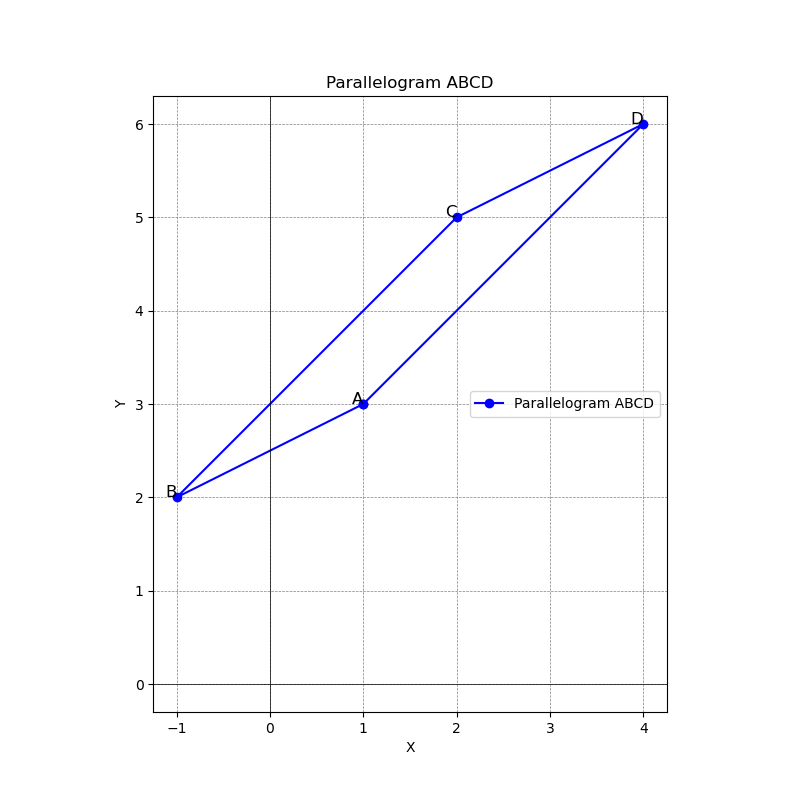
\includegraphics[width=0.7\linewidth]{figure/Figure_1.png}
	\caption{parallelogram ABCD}
\end{figure}
\end{document}

